% !TEX TS-program = pdflatex
% !TEX encoding = UTF-8 Unicode
% !TEX root = ./Abstract.tex

% This is a simple template for a LaTeX document using the "article" class.
% See "book", "report", "letter" for other types of document.

\documentclass[12pt]{article} % use larger type; default would be 10pt

% Fonts
\usepackage{times}

\usepackage{setspace}
	\doublespacing

\usepackage{textcomp}

\usepackage{textcase}
\usepackage{xcolor}


\usepackage[utf8]{inputenc} % set input encoding (not needed with XeLaTeX)

%%%%%%%%%
% Page
%%%%%%%%%

\usepackage{geometry} % to change the page dimensions
	\geometry{letterpaper} % or a4paper or letterpaper (US) or a5paper or....
	\geometry{margin=1in} % for example, change the margins to 2 inches all round
	% \geometry{landscape} % set up the page for landscape

\usepackage{graphicx} % support the \includegraphics command and options
% \usepackage[parfill]{parskip} % Activate to begin paragraphs with an empty line rather than an indent

%%% PACKAGES
\usepackage{booktabs} % for much better looking tables
\usepackage{array} % for better arrays (eg matrices) in maths

\usepackage{paralist} % very flexible & customisable lists (eg. enumerate/itemize, etc.)
\usepackage{enumitem} % Remove spacing
\setlist{nolistsep}   %     between list items

\usepackage{verbatim} % adds environment for commenting out blocks of text & for better verbatim
\usepackage{subfig} % make it possible to include more than one captioned figure/table in a single float
% These packages are all incorporated in the memoir class to one degree or another...

%%% HEADERS & FOOTERS
\usepackage{fancyhdr} % This should be set AFTER setting up the page geometry
	\pagestyle{fancy} % options: empty , plain , fancy
	\renewcommand{\headrulewidth}{0pt} % customise the layout...
	\lhead{}\chead{}\rhead{}
	\lfoot{}\cfoot{\thepage}\rfoot{}


%%% SECTION TITLE APPEARANCE
%\usepackage{sectsty}
	% \allsectionsfont{\normalfont\Large\bfseries\singlespacing} % (See the fntguide.pdf for font help) \mdseries
	% (This matches ConTeXt defaults)

\usepackage{titlesec}
	\titleformat{\chapter}[display] %[display] puts the title chapter on a separate line
		{\normalfont\huge\bfseries}{\chaptertitlename\ \thechapter}{20pt}{\Huge}
	\titleformat{\section}
		{\singlespacing\normalfont\Large\bfseries}{\thesection}{1em}{\vspace{-2ex}}
	\titleformat{\subsection}
		{\singlespacing\normalfont\large\bfseries}{\thesubsection}{1em}{\vspace{-2ex}}
	\titleformat{\subsubsection}
		{\singlespacing\normalfont\normalsize\bfseries}{\thesubsubsection}{1em}{\vspace{-2ex}}

% paragraph
%\setlength{\parskip}{1cm plus4mm minus3mm}
\setlength{\parindent}{0.5cm}

\titlespacing{\paragraph}{%
  0pt}{%              left margin
  0.5\baselineskip}{% space before (vertical)
  0.5em}%               space after (horizontal)

\usepackage{titling}
	\setlength{\droptitle}{-6em}
	\posttitle{\par\end{center}\vspace{-4em}\vskip 1em\singlespacing\normalfont}



%%% ToC (table of contents) APPEARANCE
\usepackage[nottoc,notlof,notlot]{tocbibind} % Put the bibliography in the ToC
\usepackage[titles,subfigure]{tocloft} % Alter the style of the Table of Contents
	\renewcommand{\cftsecfont}{\rmfamily\mdseries\upshape}
	\renewcommand{\cftsecpagefont}{\rmfamily\mdseries\upshape} % No bold!

% Drafting
\usepackage{draftcopy}
%	\lhead{\huge  \color{black!13} {DRAFT | DRAFT | DRAFT | DRAFT} }
%	\lfoot{\huge  \color{black!13} {DRAFT | DRAFT | DRAFT | DRAFT} }

% Comments
\usepackage{comment}

% images
\DeclareGraphicsExtensions{.pdf,.png,.jpg}
\usepackage{wrapfig}
\usepackage{float}

% Bibliography
\usepackage[font={small,it}]{caption}
\usepackage[sort&compress,comma,square,super]{natbib}         	% bibliography style

%\usepackage[colorlinks]{hyperref}    	% better urls in bibliography
\usepackage{hyperref}

\renewcommand{\refname}{\vspace{-3ex}}	% no title
\bibliographystyle{IEEEtranN}			% standard formatting, ieee
%\bibliographystyle{plainnat}			% standard formatting, ieee

%The Executive Summary presents the question asked, the methods used and the lessons learned. The summary on its own, separate from the Research Report should convey the essence of your project and should be understood by someone without scientific expertise. Do not simply replicate what you wrote in your Abstract. The difference between the Abstract and the Executive Summary is that the Executive Summary must be written in layperson (non-specialist) language. The summary will be used to explain your project to the general public and in preparing press releases for the media.

%The Executive Summary must be double-spaced and use 12 point or larger Arial or Times New Roman font. No identifying information, such as name, high school or references to gender or research facilities should be included.

%The Executive Summary may not exceed one page and is not included in the 18-page limit for the Research Report


\newcommand{ \titleText } {Post-Disaster Recovery by Rapid High Resolution Aerial Imaging and Indoor 3D Mapping with Autonomous Quadrotor UAVs driven by Computer Vision Feature Targeting and Real-time Victim Recognition}

\title{Executive Summary}
\chead{\footnotesize \normalfont \parbox{16cm} {\centering{\textbf{\textsc{ \textrm{ \titleText } }}}} }
\cfoot{}
%\author{\vspace{0ex}}
\date{\vspace{-12ex}}

\begin{document}
%\maketitle
\section*{Executive Summary}
\thispagestyle{fancy}



\noindent
\textbf{We built an autonomous drone for under \$500 to help save thousands of victims of floods, earthquakes, hurricanes and other disasters by automatically searching for victims, both indoors and outdoors.}
Our drone produces aerial maps that are \textit{10 times higher resolution} than the best commercial satellite maps in the market, allowing disaster responders to \textbf{prioritize search and rescue efforts and assess the extent of damage after a disaster}. Victims are automatically recognized by the drones and are tagged for rescue. Each drone collaborates with other drones in its network to map a city rapidly.

\noindent
A version of the drone can navigate around the inside of a building, producing a 3D map of the interior of a building that may be too dangerous to enter. A victim inside a collapsing building can be located, potentially saving the life of an EMT or firefighter.

\noindent
Recent disasters where this technology would have been applicable to post-disaster response are Hurricane Sandy, the Fukushima Nuclear Disaster and the Boston Marathon bombing by automatically searching for victims, entering a radioactive hazard zone or searching for the perpetrators.

\begin{figure}[h]
	\begin{minipage}{.55\textwidth}
		 \caption{Panoramic image from above rooftops}
		 \label{fig:StellingStitch}
		 \centering
		 	\includegraphics[width=.95\linewidth]{illustrations/maps/stelling}
	\end{minipage}
	\begin{minipage}{.45\textwidth}
 		\caption{Generated 3D indoor model}
 		\label{fig:BedPointCloud}
 		\centering
 			\includegraphics[width=.95\linewidth]{illustrations/clouds/bed2}
	\end{minipage}
\end{figure}

%\begin{figure}[h]
%	\begin{minipage}{.55\textwidth}
%	\caption{Map created from house flyover}
%	\label{fig:HouseStitch}
%	\centering
%		\includegraphics[width=.95\linewidth]{illustrations/maps/house}
%	\end{minipage}
%	\begin{minipage}{.45\textwidth}
%		 \caption{Panoramic image from above rooftops}
%		 \label{fig:StellingStitch}
%		 \centering
%		 	\includegraphics[width=.95\linewidth]{illustrations/maps/stelling}
% 		\caption{Generated 3D indoor model}
% 		\label{fig:BedPointCloud}
% 		\centering
% 			\includegraphics[width=.95\linewidth]{illustrations/clouds/bed2}
%	\end{minipage}
%\end{figure}

\begin{figure}[H]
  \caption{Full panorama from a backyard sweep}
  \label{fig:BackyardPanoStitch}
  \centering
    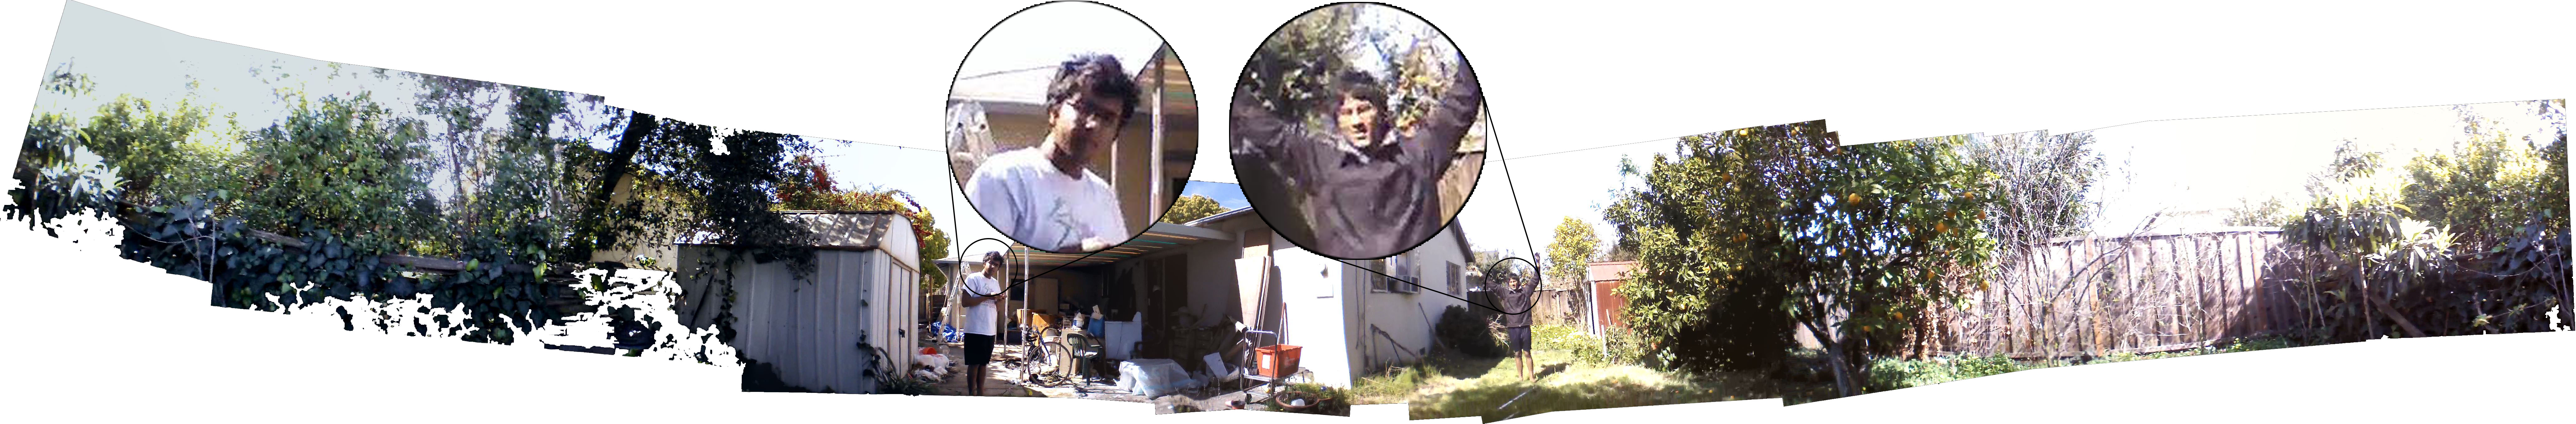
\includegraphics[width=\textwidth]{illustrations/maps/backyard_pano_mag}
\end{figure}

\end{document}